\lab{Lorenz Equations}{Lorenz Equations}
% \epigraph{\textit{Chaos: When the present determines the future, but the approximate present does not approximately determine the future.}}{Edward Lorenz}
\objective{Investigate the behavior of a system that exhibits chaotic behavior.
Demonstrate methods for visualizing the evolution of a system.}

Chaos is everywhere.
It can crop up in unexpected places and in remarkably simple systems, and a great deal of work has been done to describe the behavior of chaotic systems.
One primary characteristic of chaos is that small changes in initial conditions result in large changes over time in the solution curves.

\section*{The Lorenz System}
One of the earlier examples of chaotic behavior was discovered by Edward Lorenz.
In 1963, while working to study atmospheric dynamics he derived the simple system of equations
\begin{align*}
\frac{\partial x}{\partial t} &= \sigma \left(y - x\right) \\
\frac{\partial y}{\partial t} &= \rho x - y - x z \\
\frac{\partial z}{\partial t} &= x y - \beta z
\end{align*}
where $\sigma$, $\rho$, and $\beta$ are all constants.
After deriving these equations, he plotted the solutions and observed some unexpected behavior.
For appropriately chosen values of $\sigma$, $\rho$, and $\beta$, the solutions did not tend toward any steady fixed points, nor did the system permit any stable cycles.
The solutions did not tend off toward infinity either.
With further work, he began the study of what was called a strange attractor.
This system, though relatively simple, exhibits chaotic behavior.

\subsection*{Plotting and Interacting}
We will be making interactive 3D plots using \li{matplotlib}.
Please refer back to the \textit{Introduction to Matplotlib} lab for tips and tricks to graphing 3D.
Below is some sample code to help you out.

\begin{lstlisting}
from matplotlib import rcParams, pyplot as plt
from mpl_toolkits.mplot3d import Axes3D
rcParams['figure.figsize'] = (16,10)     #Affects output size of graphs.
'''
Code up your X, Y, Z values
'''
fig = plt.figure()
ax = fig.gca(projection='3d')
ax.plot( X, Y, Z )    #Make sure X, Y, Z are same length.
                      #Connect points (X[i], Y[i], Z[i]) for i in len(X)
ax.set_xlabel('X')
ax.set_ylabel('Y')
ax.set_zlabel('Z')

ax.set_xlim3d([min(X), max(X)])    #Bounds the axes nicely
ax.set_ylim3d([min(Y), max(Y)])
ax.set_zlim3d([min(Z), max(Z)])

plt.show()
\end{lstlisting}

Because we are plotting in 3D, we are also interested in being able to interact with the plot and rotate it to analyze what our solutions are actually doing.
To facilitate this, \li{matplotlib} has different backends which allow for various levels of control over what our graphs do.
These backends are accessed using \li{matplotlib}'s \li{switch_backend()} function with a call to whichever backend we want.
Your computer may default to a backend which you can already interact with (try clicking your plot and rotating it to see).
If not, consider using 'qt5agg', 'qt4agg', nbagg', or 'tkagg' in the function call.

\begin{lstlisting}
plt.switch_backend('qt5agg') # This backend opens the graph in a new window
\end{lstlisting}

\begin{warn}
Do not run \li{\%matplotlib inline} with this code. You will crash your kernel.
\end{warn}

\begin{problem}
Solve and graph the Lorenz equation by completing the code.
Initialize the initial conditions with random values between $-15$ and $15$.
For this exercise, let $\sigma=10$, $\rho=28$, $\beta=\frac{8}{3}$.
Compare to Figure \ref{fig:Single_Lorenz}
\begin{lstlisting}
import numpy as np
from scipy.integrate import odeint

def lorenz_ode(inputs, T):
	'''
	Code up the sytem of equations given
	'''
	return Xprime, Yprime, Zprime

def solve_lorenx(init_cond, time=10):
	T = np.linspace(0, time, time*100)	#initialize time interval for ode
	'''
	Use odeint in conjuction with lorenz_ode and the time interval T
	To get the X, Y, and Z values for this system.
	You will need to transpose the output of odeint to graph it correctly.
	'''
 	return X, Y, Z

sigma = 'value'
rho = 'value'
beta = 'value'
init_cond = [x0, y0, z0]

X, Y, Z = solve_lorenz(init_cond, 50)
'''
Code to graph
'''
\end{lstlisting}

\end{problem}


\begin{figure}
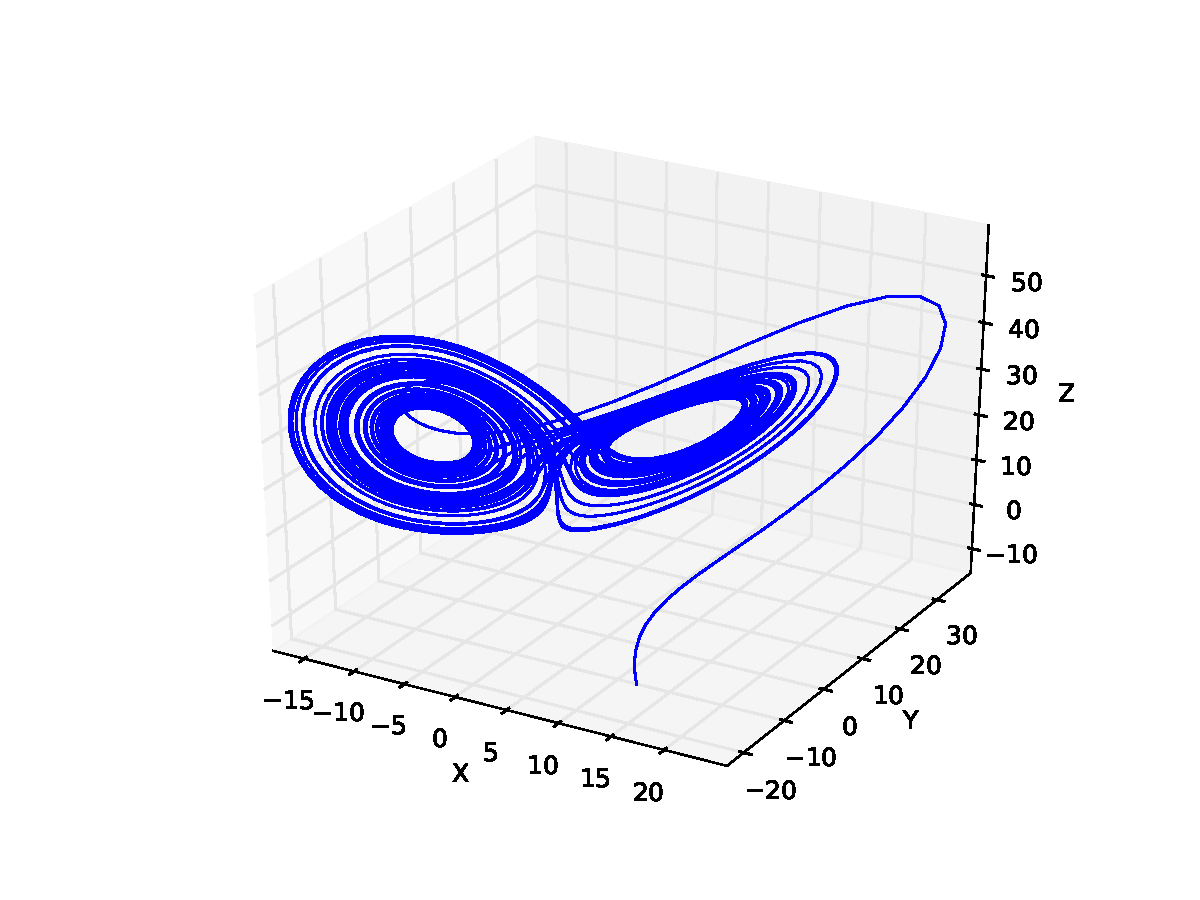
\includegraphics[width=\textwidth]{figures/Single_Lorenz.pdf}
\caption{Approximate solution to the Lorenz equation with random initial conditions}
\label{fig:Single_Lorenz}
\end{figure}

\section*{Basin of Attraction}
Notice in the first problem that the solution tended to a 'nice' region.
This region is a basin of attraction, and the set of numerical values towards which a system will converge to is an \textbf{attractor}.
Consider what happens when we change up the initial conditions.
\begin{problem}
Change your code to plot $n$ different solution using different random initial conditions.
Produce a plot with $n=3$ different solutions.
Compare to Figure \ref{fig:Multiple_Lorenz}
\end{problem}

\begin{figure}
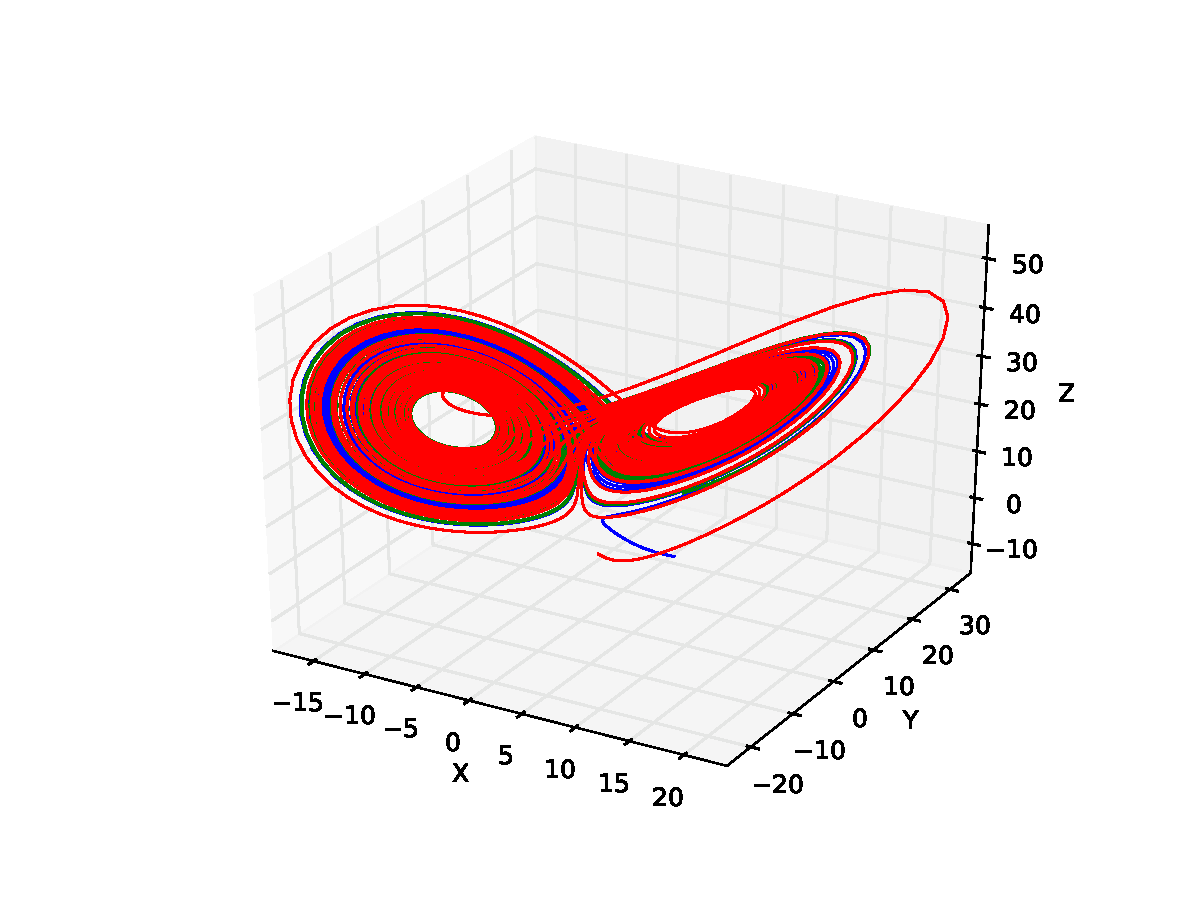
\includegraphics[width=\textwidth]{figures/Multiple_Lorenz.pdf}
\caption{Multiple solutions to the Lorenz equation with random initial conditions}
\label{fig:Multiple_Lorenz}
\end{figure}

\section*{Chaos}

Chaos in dynamical systems connotes a high sensitivity to initial conditions.
Small differences in initial conditions can yield widely diverging outcomes for these systems.
Despite having equations that completely determine the future behavior of systems, there is no way to determine where a system will be time $t$ down the road without running through the full interval.
In other words, these systems are unpredictable.

\begin{problem}
Change the code above so that it initializes one set of initial conditions and creates a second set of initial conditions by adding the array \li{np.random.randn(3)*(1E-10)}.
This will represent a small perturbation in the initial conditions. Make sure the \li{time} variable is large enough to notice a difference in the two solutions.
Plot both solutions together.
Refer to Figure \ref{fig:perturbed_lorenz}
\end{problem}

\begin{figure}
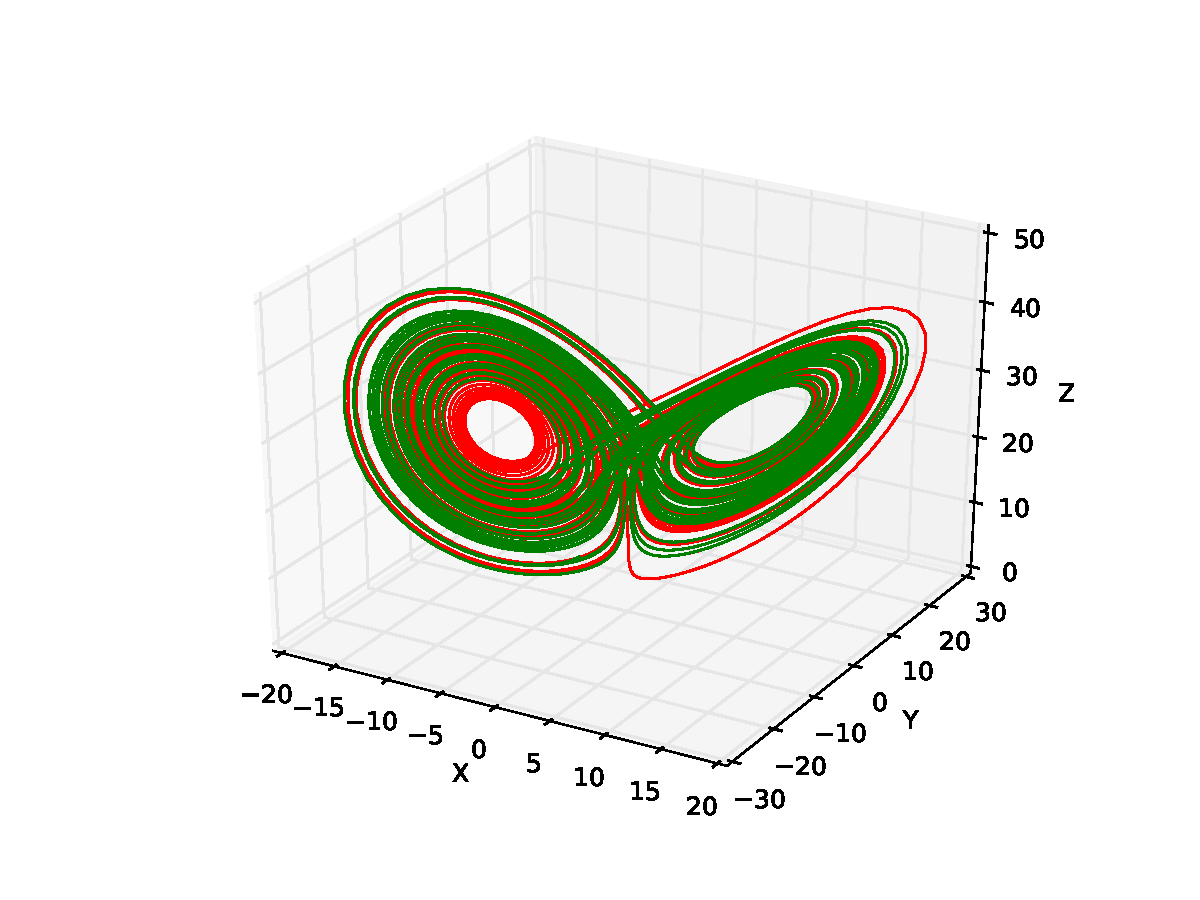
\includegraphics[width=\textwidth]{figures/perturbed_lorenz.pdf}
\caption{Two solutions to the Lorenz equation with perturbed initial conditions}
\label{fig:perturbed_lorenz}
\end{figure}

You may be wondering if your code was even correct.
You could distinctly see the two curves because there was some separation of color, but who is to say that the two solutions moved away from each other only slightly as time went on.
Our next task will be to \textit{animate} this beast.

\section*{Intro to Animation}
Let's get you a degree in Computer Animation.
You will be provided with some code that helps with animation.
Please feel free to play around and try to animate different things.
Again, refer to the \textit{Introduction to Matplotlib} lab for additional help.

We will call on \li{matplotlib.animate} to assist in animation. Import the following:
\begin{lstlisting}
from matplotlib.animation import FuncAnimation
\end{lstlisting}
Follow these steps for setting up an animation.
\begin{itemize}
\item Calculate all data needed for the animation (not necessary in some cases, but it simplifies things).
\item Define a figure explicitly with \li{plt.figure()} and set its window boundaries.
\item Draw empty objects that can be altered dynamically.
\item Define a function to update the drawing objects.
\item make a call to \li{FuncAnimation()} which will start the animation.
\end{itemize}
\li{FuncAnimation()} accepts the figure to be animated, the function that updates the figure, the number of frames to show before repeating, and how fast to run the animation (lower number $=$ faster).

Check out the sample code for animating two 2D objects simultaneously.
\begin{lstlisting}
from matplotlib.animation import FuncAnimation

def sine_cos_animation():
	#Calculate the data to be animated
	x = np.linspace(0, 2*np.pi, 200)[:-1]
	y1, y2 = np.sin(x), np.cos(x)
	
	#Create a figure and set the window boundaries
	fig = plt.figure()
	plt.xlim(0, 2*np.pi)
	plt.ylim(-1.2, 1.2)
	
	#Initiate empty lines of the correct dimension
	sin_drawing, = plt.plot([], [])
	cos_drawing, = plt.plot([], [])	#note the comma after the variable name
	
	#Define a function that updates each line
	def update(index):
		sin_drawing.set_data(x[:index], y1[:index])
		cos_drawing.set_data(x[:index], y2[:index])
		return sin_drawing, cos_drawing,
	
	a = FuncAnimation(fig, update, frames=len(x), interval=10)
	plt.show()
\end{lstlisting}

\begin{warn}
The above animation code works great for 2D animations, but \li{set_data()} is only good for 2D. When you want to animate in 3D, you will need an extra empty list in \li{plt.plot()} and a call to \li{set_3d_properties()} in the \li{update(index)} function.
\end{warn}

\section*{Animate}
You now know how to plot the Lorenz equation, how to plot multiple equations, and even how to animate (yay you, you're a star) simple plots.
It's time to put all your know-how to good use.

\begin{problem}
Animate the solutions of the Lorenz equation for an initial set of conditions and the perturbed conditions on the same plot.
To make the animation go faster, decrease the \li{interval} value in the \li{FuncAnimation()} call.
It will take several seconds before the curves split, so be patient.
\end{problem}

If our system is very chaotic, then even small round off errors in your computer can lead to drastically different solutions.

\begin{problem}
Now set one initial condition.
Use \li{odeint} to solve the system, but use the arguments \li{atol=1E-14}, \li{rtol=1E-12}, and then again with \li{atol=1E-15}, \li{rtol=1E-13}.
Animate both solutions on the same plot.
\end{problem}

\section*{Lyapunov Exponents}
The Lyapunov exponent of a dynamical system is one measure of how chaotic a system is.
While there are more conditions for a system to be considered chaotic, one of the primary indicators of a chaotic system is \emph{extreme sensitivity to initial conditions}.
Strictly speaking, this is saying that a chaotic system is poorly conditioned.
Usually, in dynamical systems, the sensitivity to changes in initial conditions depends exponentially on the time the system is allowed to evolve.
If $\delta(t)$ represents the difference between two solution curves, when $\delta(t)$ is small, the following approximation holds.
\[\|\delta(t)\| \sim \|\delta(0)\| e^{\lambda t}\]
where $\lambda$ is a constant called the Lyapunov exponent.
For the Lorenz system, experimentally it can be verified that $\lambda \approx .9$.

\begin{figure}
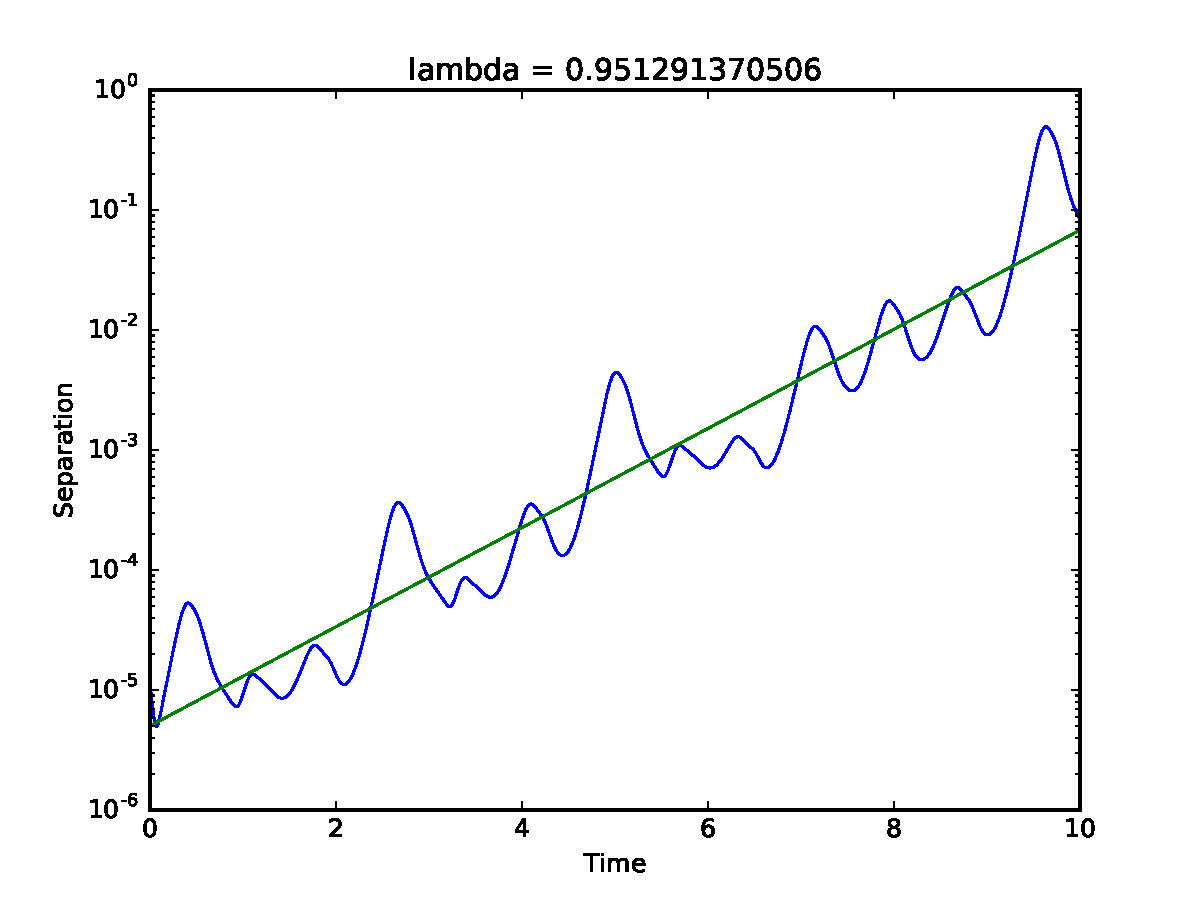
\includegraphics[width=\textwidth]{figures/semilog.pdf}
\caption{A semilog plot of the separation between two solutions to the Lorenz equations together with a fitted line that gives a rough estimate of the Lyapunov exponent of the system.}
\label{fig:lyapunov_exponent}
\end{figure}

Suppose we want tol find the Lyapunov exponent for the Lorenz System.
Start by importing \li{linalg} and \li{linregress} modules from \li{scipy}.
\begin{lstlisting}
from scipy import linalg as la
from scipy.stats import linregress
\end{lstlisting}
To get a good estimate of the Lyapunov exponent, we want to make sure our initial solution already lies on the attractor.
To do this, choose some random initial conditions, run your \li{solve_lorenz} function, then pick out the final coordinates.
Let these coordinates be the starting point for our next system.

Next perturb the conditions slightly.
Find the solution curve using these two sets of initial coordinates and then calculate the \li{norm} between the solution at each point.
Plot the norm using \li{plt.semilogy(time, norm)}.

Finally we want to calculate the exponential line fitted to the data.
Because we are using the semilog plot, we can find this line as follows:
\begin{itemize}
\item take the \li{log} of the norms.
\item use \li{linregress()} to compute the linear regression of the log of the norms.
\item take the \li{exp} of the linear regression to turn back into an exponential regression.
\item plot the exponential regression using \li{plt.semilogy()} (your solution will be a line)
\end{itemize}


\begin{problem}
Write a Python function that finds an initial point on the strange attractor, runs the simulation to a given time $t$, and produces a semilog plot of the norm of the difference between the two solution curves.
Also have it plot an exponential line fitted to match the curve (this will be linear on the semilog plot).
Have it return a rough estimate of the Lyapunov exponent.
The output should be something like Figure \ref{fig:lyapunov_exponent}.

Note: In order to get a good estimate of the Lyapunov exponent, your initial guess should already lie on the strange attractor.
You can get a value on the attractor by running the system for a while to find a good initial guess.

Hint: To find the fitting line, take the logarithm of the norms of the differences, compute a linear fit, then take the exponential function of the resulting line.
The Lyapunov exponent will be approximately equal to the slope found by the linear regression.
\end{problem}